\documentclass[11pt]{article}
\usepackage[margin=1in]{geometry}
\usepackage{amsmath,amssymb}
\usepackage{booktabs}
\usepackage{graphicx}
\usepackage{hyperref}
\usepackage{xcolor}
\usepackage{authblk}
\usepackage[round]{natbib}
\hypersetup{colorlinks=true,linkcolor=blue,citecolor=blue,urlcolor=blue}

\title{\bfseries When Do Audited Action Gates Help?\\
The Cost and Failure Conditions of Epistemic Strictness\\ in LLM Agents}

\author[1]{Rong Xiang}
\affil[1]{Independent researcher}
\date{\today}

\begin{document}
\maketitle

\begin{abstract}
Recent work equips LLM agents with mechanisms that verify internal beliefs before
committing to actions, and reports that such mechanisms improve faithfulness. We ask
the complementary question: \emph{what do these mechanisms cost, and when do they fail?}
We build a synthetic fault-diagnosis environment in which genuine causal rules and
constructed spurious associations are indistinguishable from observation and separable
only by intervention, so that epistemic strictness carries a real price. Across
$1{,}330$ completed agent runs on nine models we report four findings.
(i)~Increasing strictness suppresses superstition and discovery together: spurious-rule
adoption falls by $1.51$ of $4$ and true-rule recall by $0.111$ (paired, $n{=}57$,
Holm-corrected $p<0.02$), but the size of the discovery cost varies sharply across
models, so there is no single model-independent frontier.
(ii)~Self-reported epistemic status is unreliable: agents label rules \textsc{verified}
whose causal component was never intervened upon, and a gate that trusts those labels
yields no detectable benefit, whereas a harness-audited gate does.
(iii)~Restricting action to audited rules improves downstream diagnosis by
$+0.114$ $[+0.019,+0.208]$ ($n{=}55$ paired, four models, held-out evaluation half),
but the benefit is concentrated almost entirely in systems that were already performing
poorly: $+0.31$ when the ungated baseline is below $0.60$ versus $+0.01$ at
$0.80$--$0.95$ (independent-covariate design, $r{=}-0.537$, permutation $p{=}0.0007$).
(iv)~The gate's effect \emph{changes sign} with the verification budget: with no budget
it \emph{reduces} accuracy by $0.315$, and the budget-by-gate interaction
($\mathrm{DiD}=+0.456$ $[+0.297,+0.625]$) is the largest effect we measure.
We also refute our own pre-registered hypothesis that over-strict agents stop exploring:
intervention usage is flat across six strictness levels. An audited action gate does not
make an agent smarter; it prevents a belief set already contaminated by coincidences from
degrading action---and only when the system can afford to verify.
\end{abstract}

\section{Introduction}

A recurring assumption in work on LLM agents is that more caution is better: an agent that
abstains under uncertainty, or that verifies its beliefs before acting, is treated as
strictly improved. The tendency to propose causal hypotheses on limited evidence, however,
drives two things at once: the adoption of coincidences (false positives) and the discovery
of genuine but not-yet-confirmed rules (true positives). If both are driven by the same
disposition, suppressing one should suppress the other.

The abstention literature has quantified a related trade-off in question answering, where
over-abstention reduces usefulness on questions the model could have answered. That is not
the trade-off studied here. Our cost lands on a different quantity: the \emph{discovery of
new causal rules} in an interactive setting where the agent must decide whether to spend a
budget on experiments.

\paragraph{Why a synthetic environment.} Testing this requires an environment in which
(a)~genuine rules and spurious associations are indistinguishable in observational data,
(b)~only intervention separates them, and (c)~ground truth is known by construction so that
no human annotation is needed. Natural corpora do not satisfy all three.

\paragraph{Pre-registered hypotheses.} We fixed three hypotheses before collecting data.
\textbf{T1} (trade-off): raising strictness lowers both spurious adoption and true-rule
discovery. \textbf{T2} (mechanism): separating \emph{holding} a hypothesis from
\emph{acting} on it pushes the frontier outward. \textbf{T3} (non-monotonicity): an
over-strict agent stops exploring and discovery collapses. Section~\ref{sec:results}
reports which survived; Appendix~\ref{app:refuted} lists every hypothesis of our own that
the data refuted.

\paragraph{Contributions.} We do not propose a new mechanism. Verification-before-commitment
and auditable hypothesis protocols already exist \cite{saver,hep}, as do synthetic
interactive causal-discovery environments \cite{causalab,interventional}. Existing work
reports that such mechanisms work. We measure what they cost and when they stop working:

\begin{enumerate}\itemsep2pt
\item a quantified discovery cost of epistemic strictness, and evidence that its magnitude
is model-dependent rather than universal (\S\ref{sec:t1});
\item evidence that model-\emph{self-reported} epistemic status is systematically
unfaithful, so gates built on self-labels are ineffective, while gates built on
harness-side interventional audit are not (\S\ref{sec:labels});
\item the moderation structure of the gate's benefit, measured with a split-half design
that removes the shared-noise artefact (\S\ref{sec:t2});
\item a sign-flipping budget-by-gate interaction: without verification budget, the gate is
harmful (\S\ref{sec:interaction});
\item full release of code, environment, per-run checkpoints and prompts.
\end{enumerate}

\section{Related work}

\paragraph{Abstention.} \citet{agentabstain} build a paired-task benchmark for agentic
abstention across $42$ sandbox environments and $17$ frontier models, and report that
abstention capability is largely independent of general task-solving capability.
\citet{agenticabstention} treat abstention as a sequential decision and evaluate $13$ agent
systems on more than $28{,}000$ tasks. These works measure whether an agent abstains when it
should; we measure what strictness costs on the discovery side.

\paragraph{Verification before action.} \citet{saver} propose SAVeR, which enforces
verification over internal belief states before action commitment via adversarial
self-auditing, and report improved faithfulness \emph{while preserving competitive
end-task performance}. The Hypothesis Evolution Protocol \citep{hep} makes hypothesis generation, evaluation
and evolution explicit and auditable, and reports that stronger base models exploit the
protocol more fully. Our audit differs in
substrate: SAVeR checks internal logical and evidential consistency using the model itself,
whereas our gate checks each rule against \emph{external interventional records} produced by
the harness, which the model cannot fabricate. Our data bear directly on the self-auditing
assumption (\S\ref{sec:labels}), and our moderation result stands in tension with
that capability finding (\S\ref{sec:discussion}).

\paragraph{Interactive causal discovery.} CausaLab \citep{causalab} places agents in a synthetic
laboratory with prior records and budgeted interventions, and reports a persistent gap
between task accuracy and mechanism recovery. Related work argues that progress
should be measured by interventional outcomes against a fixed hidden structural causal model
rather than by the agent's own narrative \citep{interventional}. Our environment shares the budgeted-intervention
setting; it differs in that the confounding structure is \emph{fixed by construction}, so a
specific set of $M$ spurious pairs is known in advance and ``spurious-rule adoption'' can be
used directly as a dependent variable.

\paragraph{Memory and propagation.} \citet{trajectory} show that spurious correlations
persisted in agentic memory become self-reinforcing, because the actions they induce
generate the next trajectory written back to memory. \citet{governedmemory} formalise
shared-memory failure modes including provenance collapse. These lines concern propagation
across steps and agents; the present paper concerns the genesis of spurious belief within a
single agent.

\section{The Fault World environment}

\subsection{Structure}
A synthetic machine is described by components and symptoms named with random
semantics-free symbols, re-randomised for every run to exclude memorisation. The base
configuration has $6$ components and $8$ symptoms, giving a hypothesis space of $48$
candidate rules:

\begin{itemize}\itemsep2pt
\item $K{=}3$ \emph{true causes}: component $c_i$ causes symptom $s_i$ with $P=0.90$;
baseline occurrence without the cause is $0.05$.
\item $2$ \emph{confounded components}: each is driven by a hidden latent $Z$ that also
drives two symptoms, producing $M{=}4$ \emph{spurious pairs}.
\item one pure-noise component and one pure-noise symptom.
\end{itemize}

\subsection{The invariant that makes strictness costly}
Table~\ref{tab:invariant} reports $20{,}000$-sample checks. Observationally, spurious pairs
look like moderately strong rules; under intervention they collapse to the $0.5$ base rate
while true rules are unchanged. An agent therefore cannot separate them without spending
intervention budget.

\begin{table}[t]\centering
\caption{Environment invariant ($20{,}000$ samples, base configuration).}
\label{tab:invariant}
\begin{tabular}{lcc}
\toprule
Relation & Observational $P(s\mid c{=}1)$ & Interventional $P(s\mid do(c{=}1))$\\
\midrule
True rules ($K{=}3$)      & $0.902,\ 0.904,\ 0.897$ & $0.902,\ 0.903,\ 0.899$\\
Spurious pairs ($M{=}4$)  & $0.773,\ 0.740,\ 0.777,\ 0.740$ & $0.503,\ 0.496,\ 0.497,\ 0.502$\\
\bottomrule
\end{tabular}
\end{table}

\subsection{Parameterised variants}
For robustness we vary the generative parameters: \textsc{weak} (observational
co-occurrence $0.65/0.62$), \textsc{strong} ($0.86/0.83$), \textsc{rich} ($K{=}4$, $M{=}2$)
and \textsc{poor} ($K{=}2$, $M{=}6$). The interventional invariant holds in all variants.

\subsection{Agent loop}
Each run consists of three episodes. In each episode the agent receives $15$ fresh
observation logs plus the results of its previous interventions, and returns its
\emph{complete current belief set}---each rule tagged \textsc{hypothesis} or
\textsc{verified} with a confidence---together with the interventions it wishes to run.
Each intervention forces one component active or inactive and runs the machine $20$ times,
returning symptom counts. A downstream diagnostic task follows.

\section{Experimental design}

\subsection{Independent variables}
\textbf{S1, prompt-level strictness}, six levels: \textsc{l0} record anything remotely
possible; \textsc{l1} record on plausible indication; \textsc{l2} record when evidence is
reasonably consistent; \textsc{l3} record only when confident it is genuinely causal;
\textsc{l4} record only after an intervention has tested it; \textsc{l5} record only after
testing the component in both directions with a clear difference.
\textbf{S2, intervention budget}: $0/3/6/12/21$ per run.
\textbf{S4, action gate}: \textsc{off} (diagnosis may use the entire belief set),
\textsc{self} (only rules the model labelled \textsc{verified}), \textsc{audit} (only rules
that pass the harness audit).

\subsection{Harness audit criterion}
A rule $c\rightarrow e$ passes iff the run's intervention log contains either
$do(c{=}\textsc{active})$ with $e$ occurring $\geq 14/20$, or $do(c{=}\textsc{inactive})$
with $e$ occurring $\leq 6/20$. Each threshold has one-sided false-positive rate
$P(X\geq 14\mid p{=}0.5)=0.058$ against the spurious null; true rules generate $p{=}0.90$.
The model's self-reported status is treated as a measured object, never as gate input.

\subsection{Downstream task and split-half measurement}
Each diagnostic case activates exactly one true-cause component and asks which component to
repair. We use $30$ cases per run, of which typically $23$--$26$ are uniquely answerable by
an oracle holding the true rule set (a true effect fails to appear with probability $0.10$,
and two true effects sometimes co-occur; including unanswerable cases only dilutes signal---
the oracle ceiling over all cases is $0.81$).

Answerable cases are split by index parity into two disjoint halves: \textbf{A} (even),
used only to produce an \emph{independent} baseline covariate, and \textbf{B} (odd), on
which all effects are reported. This is necessary: the gate effect
$\Delta=\textsc{audit}-\textsc{off}$ shares noise with its own baseline \textsc{off}, so
without the split a moderation analysis cannot be distinguished from regression to the mean.

\subsection{Statistics}
All conditions share the same world seeds, so comparisons are paired. We report bootstrap
$95\%$ confidence intervals ($10{,}000$ resamples), $p$-values from paired sign-flip
permutation tests, and Holm--Bonferroni correction within families of contrasts. All
contrasts are reported, including non-significant ones.

\subsection{Models and fixed parameters}
Nine models were used across experiments: \texttt{qwen3.8-27b}, \texttt{glm-4.5-air},
\texttt{glm-5.2}, \texttt{kimi-k3}, \texttt{qwen3.7-flash-2026-07-15},
\texttt{qwen3.7-max-2026-06-08}, \texttt{qwen3.7-plus}, \texttt{qwen3.7-plus-2026-05-26},
\texttt{deepseek-v4-flash-0731}. The model set differs between experiments because of free
API quota availability, so results are not pooled across experiments.
Fixed parameters: chain-of-thought disabled (\texttt{enable\_thinking=false}), $15$
observations per episode, $3$ episodes, $20$ trials per intervention, temperature $1.0$.
Disabling chain-of-thought was necessary for feasibility (each call otherwise took
$60$--$150$\,s) and is an untested simplification; see \S\ref{sec:limitations}.

\section{Results}\label{sec:results}

\subsection{The environment induces superstition}
Spurious-rule adoption falls inside the pre-registered $0.15$--$0.85$ band
(belief-level mean $\approx 0.71$ at full scale). Purely observational conditions reach
$0.90$, but that is \emph{not} superstition: adopting an association when only observational
data exist is rational. The main experiments are therefore run under conditions where
intervention is available.

Illustratively, in one run the agent intervened on a confounded component and observed the
two spurious symptoms at $6/20$ and $7/20$ (versus $\approx 15/20$ observationally), yet
still recorded both spurious rules at confidence $0.7$--$0.85$, reasoning that the
intervention results were ``consistent with the primary associations'' and attributing the
deviation to randomness.

\subsection{T1: the trade-off exists, but there is no common frontier}\label{sec:t1}

\begin{table}[t]\centering
\caption{Strictness \textsc{low}$\rightarrow$\textsc{high}, three models, $n{=}57$ paired runs.}
\label{tab:t1}
\begin{tabular}{lrrl}
\toprule
Measure & $\Delta$ & $p_{\text{Holm}}$ & Verdict\\
\midrule
Spurious rules adopted (of $4$) & $-1.509$ & $.0023$ & significant\\
True-rule recall                & $-0.111$ & $.0117$ & significant\\
Interventions used              & $-0.526$ & $.108$  & \textbf{not significant}\\
Audited true rules              & $-0.029$ & $.661$  & not significant\\
\bottomrule
\end{tabular}
\end{table}

Strictness reliably suppresses superstition and also costs recall (Table~\ref{tab:t1}).
The magnitude of the cost, however, is strongly model-dependent: recall
$\Delta=-0.283$ $[-0.417,-0.150]$ for one model, versus $-0.017$ and $-0.020$ (both
unstable) for the other two. The strong form of T1---that all strictness settings lie on one
FDR--recall frontier---is \emph{not} supported: some models suppress superstition almost for
free.

\subsection{Self-reported epistemic status is unreliable}\label{sec:labels}
In one model, the high-strictness condition produced on average $1.33$ rules labelled
\textsc{verified} whose causal component had never been intervened upon at all. The effect
did not replicate in two other models ($\Delta=+0.15$ and $-0.20$, both with CIs spanning
zero), so we report it as a failure mode rather than a general claim.

Its methodological consequence is firm. Under the earlier 8-case protocol,
$\textsc{off}\rightarrow\textsc{self}$ gave $+0.090$ and
$\textsc{self}\rightarrow\textsc{audit}$ gave $+0.087$; neither survived Holm correction
($p_{\text{Holm}}=.204$), while the combined $\textsc{off}\rightarrow\textsc{audit}$ did.
Trusting self-reported labels captures at best half of the available benefit.

\subsection{T2: the gate works, but its benefit is strongly moderated}\label{sec:t2}

\begin{table}[t]\centering
\caption{Gate effect (\textsc{audit}$-$\textsc{off}) on the held-out evaluation half,
$30$-case protocol.}
\label{tab:t2}
\begin{tabular}{lrr}
\toprule
Model & $\Delta$ & $n$\\
\midrule
\texttt{deepseek-v4-flash-0731} & $+0.130$ $[-0.015,+0.260]$ & $20$\\
\texttt{glm-5.2}                & $+0.142$ $[-0.054,+0.327]$ & $20$\\
\texttt{qwen3.7-flash-2026-07-15} & $+0.065$ & $9$\\
\texttt{qwen3.7-plus-2026-05-26}  & $+0.044$ & $6$\\
\midrule
\textbf{Pooled} & $\mathbf{+0.114\ [+0.019,+0.208]}$ & $\mathbf{55}$ ($p{=}0.024$)\\
\bottomrule
\end{tabular}
\end{table}

No single model survives Holm correction (best $p_{\text{Holm}}=0.36$); the effect is
detectable only pooled (Table~\ref{tab:t2}).

The moderation is measured with the independent covariate: the $x$-axis is \textsc{off}
accuracy on development half A, the $y$-axis is the gate effect on evaluation half B, and
the two share no cases. We find $r=-0.537$, $n=55$, permutation $p=0.0007$:

\begin{center}
\begin{tabular}{lrr}
\toprule
Ungated baseline (half A) & $n$ & Gate effect (half B)\\
\midrule
$<0.60$        & $19$ & $+0.308$ $[+0.170,+0.440]$\\
$0.60$--$0.80$ & $15$ & $+0.103$ $[-0.054,+0.234]$\\
$0.80$--$0.95$ & $11$ & $+0.006$ $[-0.243,+0.216]$\\
$\geq 0.95$    & $10$ & $-0.117$ $[-0.301,+0.036]$\\
\bottomrule
\end{tabular}
\end{center}

The top bin is subject to a structural ceiling---when the baseline approaches $1.0$,
$\Delta$ can only be non-positive---and must not be read as ``the gate is harmful''. The
informative range is below $0.80$, where the benefit decays monotonically from $+0.31$ to
$+0.01$.

Crucially, when the gate helps, \emph{the belief set is not cleaner}: in the
highest-benefit conditions the agent still holds $2.5$--$3.3$ spurious rules of $4$. The
gain comes from acting more strictly, not from believing less.

\subsection{Budget by gate: without verification budget the gate is harmful}\label{sec:interaction}

\begin{table}[t]\centering
\caption{Budget $\times$ gate, two models, $20$ repetitions, $8$-case protocol.}
\label{tab:interaction}
\begin{tabular}{lrr}
\toprule
Contrast & $\Delta$ & $p_{\text{Holm}}$\\
\midrule
Gate effect at budget $0$  & $-0.315$ $[-0.452,-0.178]$ & $.0017$\\
Gate effect at budget $6$  & $+0.140$ $[+0.054,+0.227]$ & $.0080$\\
Gate effect at budget $21$ & $+0.081$ $[+0.002,+0.163]$ & $.063$\\
\midrule
Interaction (DiD), budget $0\rightarrow6$  & $\mathbf{+0.456}$ $[+0.297,+0.625]$ & $.0017$\\
Interaction (DiD), budget $0\rightarrow21$ & $+0.320$ $[+0.165,+0.477]$ & $.0017$\\
\bottomrule
\end{tabular}
\end{table}

With zero budget the audited set is necessarily empty, so the gate strips the agent of every
usable rule; one model falls to $0.28$ accuracy. The interaction
(Table~\ref{tab:interaction}, Figure~\ref{fig:interaction}) is the largest effect we measure
and explains the main effect: the gate helps because the audited set contains something, and
the audited set contains something because budget was spent.

\begin{figure}[t]\centering
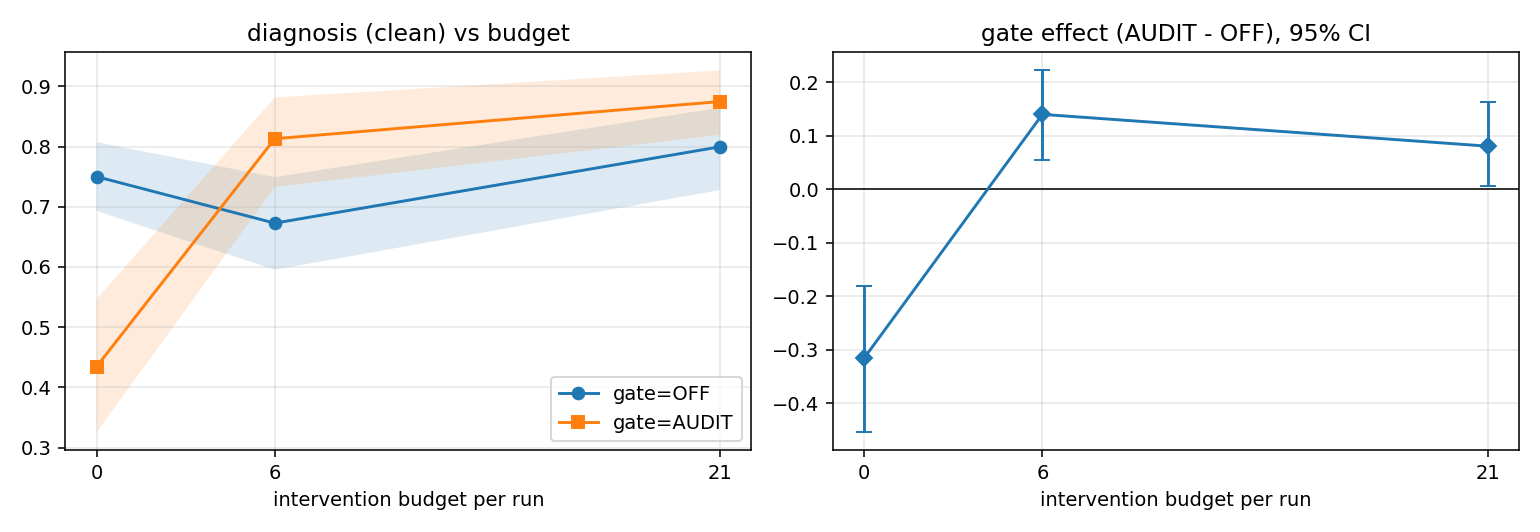
\includegraphics[width=\textwidth]{figs/bg_interaction.png}
\caption{Left: downstream accuracy under both gate settings as a function of intervention
budget. Right: the gate effect with $95\%$ CIs; the sign flips between budget $0$ and $6$.}
\label{fig:interaction}
\end{figure}

\subsection{Budget is not a strictness dial}
Raising the budget from $0$ to $21$ leaves spurious adoption essentially unchanged (only one
adjacent step survives correction, and the next step reverses) and leaves recall unchanged.
What grows is the number of \emph{audited} rules ($0\rightarrow3.35$--$3.65$;
Figure~\ref{fig:s2}). Giving an agent more opportunities to verify does not stop it
believing coincidences; it only increases the stock of evidence available to the action
layer. This reinforces the mechanism reading of \S\ref{sec:t2}.

\begin{figure}[t]\centering
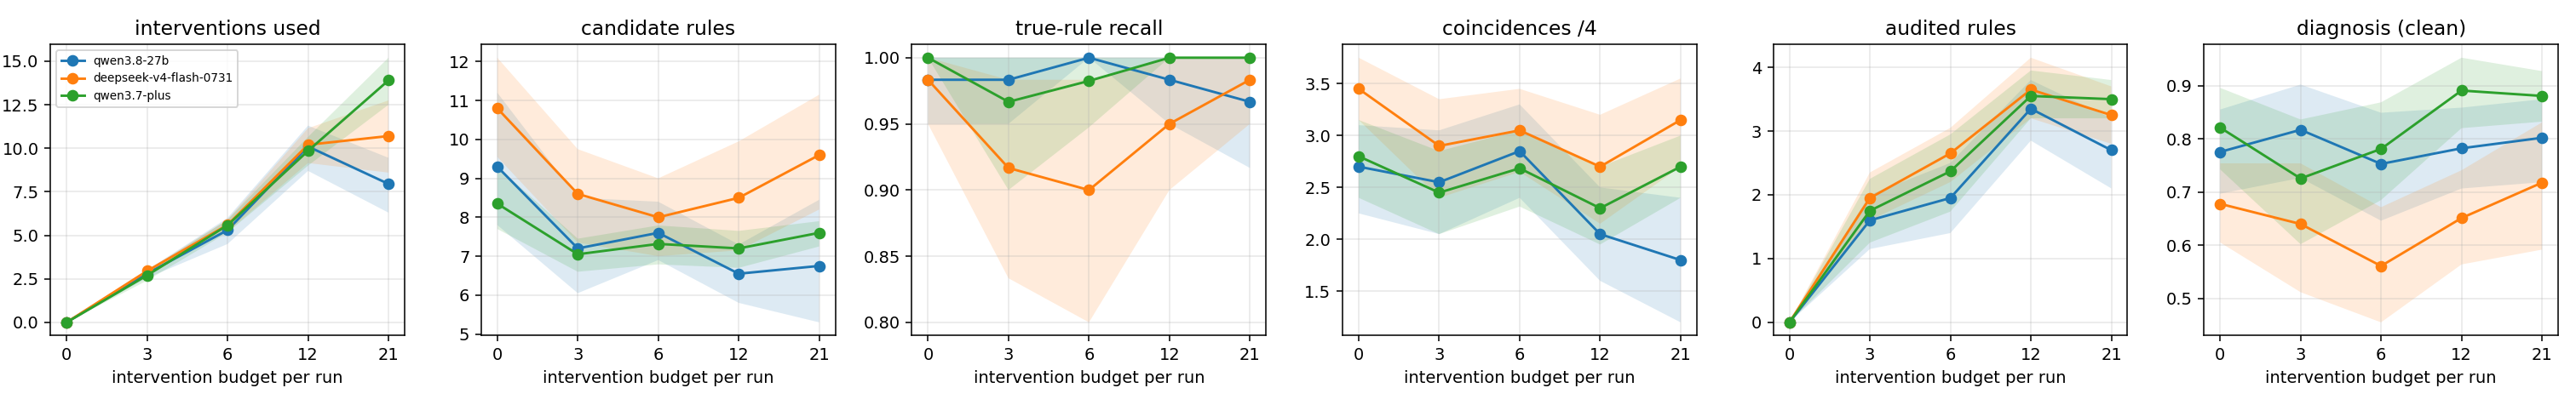
\includegraphics[width=\textwidth]{figs/s2_curves.png}
\caption{Intervention budget ladder. Belief-level spurious adoption is flat; audited rules
grow with budget; budget stops binding above $12$.}
\label{fig:s2}
\end{figure}

\subsection{T3 refuted: strict agents do not stop exploring}
Across six strictness levels and three models, intervention usage stays at the budget
ceiling ($4.80$--$6.00$, $5.85$--$6.00$, $6.00$), and exploration breadth does not collapse.
Every adjacent contrast on intervention count has $p_{\text{Holm}}>0.29$.

A discovery cliff does exist, but not where T3 predicted. Per-level recall loss is
essentially zero from \textsc{l0} to \textsc{l2}; it appears at
$\textsc{l3}\rightarrow\textsc{l4}$ ($-0.091$, $p_{\text{Holm}}=.088$, marginal) and
$\textsc{l4}\rightarrow\textsc{l5}$ ($-0.152$, $p_{\text{Holm}}=.048$). The cliff is located
where the requirement changes from subjective confidence to an objective evidential
threshold, not at the far end of a verbal strictness scale. The four purely verbal levels
\textsc{l0}--\textsc{l3} are nearly free: candidate rules fall from $28.9$ to $5.95$ in one
model while recall drops only $0.05$. Prompt-level strictness mostly removes redundant
candidates, not discovery capability (Figure~\ref{fig:t3}).

\begin{figure}[t]\centering
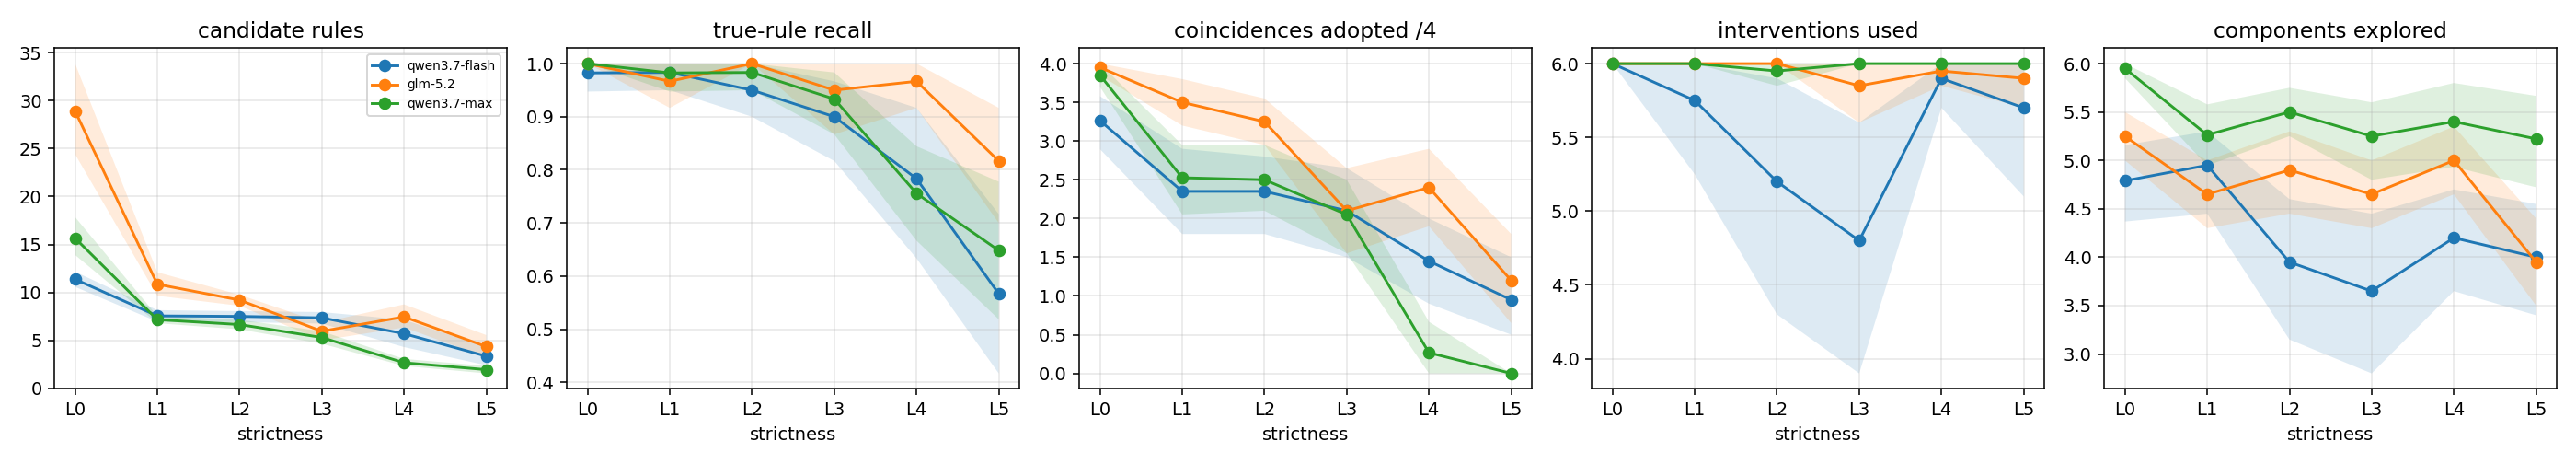
\includegraphics[width=\textwidth]{figs/t3_curves.png}
\caption{Strictness ladder. Interventions used (fourth panel) is flat, refuting the
exploration-collapse hypothesis; the recall cliff appears only at \textsc{l4}--\textsc{l5}.}
\label{fig:t3}
\end{figure}

\subsection{Robust to the environment, sensitive to the model}
On a previously unused model, across all five environment variants including the one
equivalent to the main experiments, the pooled gate effect is
$+0.006$ $[-0.077,+0.088]$, $n=40$, with no variant significant. Spurious adoption tracked
the environment as designed ($1.6/4$ under \textsc{weak} to $3.9/4$ under \textsc{strong}),
so the manipulation worked. The result is robust to environment parameters and not robust to
model choice. Under the moderation structure of \S\ref{sec:t2} this non-replication is
expected: that model's baseline was $0.78$--$0.90$, inside the zero-benefit region.

\section{Discussion}\label{sec:discussion}

\paragraph{Caution is not free, and not uniformly expensive.} Strictness reliably suppresses
superstition. It costs recall, and in some models a great deal of it, but the cost is not
universal, and verbal strictness is cheap over a wide range. What is expensive is the step
from ``be confident'' to ``have interventional evidence''.

\paragraph{What an action gate actually does.} It does not make the agent smarter. In the
conditions where it helps most, the belief set still contains three spurious rules of four;
the gate severs the path from those rules to action. Two conditions follow, and both are
engineering-relevant: the gate requires that the system can already verify (at zero budget
it costs $0.315$ accuracy), and it requires that the system is not already performing well
(benefit $+0.31$ below baseline $0.60$ versus $+0.01$ at $0.80$--$0.95$).

\paragraph{Tension with capability-scaling results.} The Hypothesis Evolution Protocol
\citep{hep} reports that stronger base models exploit an auditable hypothesis protocol
\emph{more} fully, whereas we find the gate's
accuracy benefit \emph{shrinks} as the ungated baseline rises. The measured quantities
differ---protocol utilisation versus downstream accuracy gain---and we cannot resolve the
tension with our data, but the two should not be conflated. It is possible for a strong model
to use a protocol more thoroughly while gaining less from it.

\paragraph{A negative result worth stating.} Giving an agent more chances to verify does not
make it stop believing coincidences. Budget changes the evidence stock, not the belief set.
This suggests the belief layer and the evidence layer are only weakly coupled in current
LLM agents, which is precisely why an action-side gate, rather than a belief-side
intervention, is the effective lever.

\section{Limitations}\label{sec:limitations}
\begin{enumerate}\itemsep2pt
\item Chain-of-thought was disabled throughout. Whether these conclusions hold with reasoning
enabled is untested.
\item The model set differs between experiments because of quota availability, and some cells
are small (minimum $6$ paired observations). Results are not pooled across experiments.
\item No single model survives Holm correction for the T2 main effect; it is detectable only
in the pooled sample.
\item The split-half is a fixed parity split rather than a randomised one.
\item The budget-by-gate interaction was measured under the earlier $8$-case protocol and,
by analogy with \S\ref{sec:t2}, its magnitude is probably overestimated.
\item Five environment variants were tested but all belong to one generative family; non-binary
symptoms, temporal dependence and multi-cause interactions are untested.
\item Models used are mid-sized and inexpensive; frontier models are untested.
\end{enumerate}

\section{Reproducibility}
Code, data and per-run records are available at
\url{https://github.com/aiegisafety/fault-world}.
Every run is checkpointed with its complete conversation, executed interventions and
diagnostic answers, so all reported numbers can be recomputed from raw records without
API access. The release contains the environment (\texttt{fault\_world\_v2.py},
\texttt{fault\_world\_v3.py}), the step-wise resumable experiment driver
(\texttt{run\_2x2.py}), the audit and oracle code (\texttt{audit\_gate.py}), and the analysis
scripts (\texttt{analyze\_2x2.py}, \texttt{stats.py}, \texttt{holm.py}, \texttt{t3\_curve.py},
\texttt{s2\_curve.py}, \texttt{bg\_interaction.py}, \texttt{e4\_robustness.py},
\texttt{t2\_replication.py}). In total $1{,}330$ runs completed across $18$ experiment cells.

\appendix
\section{Hypotheses of ours that the data refuted}\label{app:refuted}

\begin{center}
\begin{tabular}{p{0.45\textwidth}p{0.45\textwidth}}
\toprule
Original hypothesis & Outcome\\
\midrule
Over-strict agents stop exploring (T3) & Refuted: intervention usage flat across six levels\\
A single model-independent FDR--recall frontier exists & Not supported: the cost is model-dependent\\
Prompt-level strictness is the primary independent variable & Downgraded: \textsc{l0}--\textsc{l3} nearly free\\
Self-reported \textsc{verified} labels can be trusted & Refuted: must be audited by the harness\\
Strictness induces Goodharting of status labels & Not replicated: single-model observation\\
Intervention budget is a form of strictness & Refuted: it only grows the evidence stock\\
The action gate extends the frontier unconditionally & Conditional: harmful at zero budget\\
The gate's benefit is general & Conditional: strongly moderated by the ungated baseline\\
Strictness reduces intervention count & Withdrawn after Holm correction ($p=.108$)\\
Evidential requirements increase exploration & Withdrawn after Holm correction ($p=.294$)\\
\bottomrule
\end{tabular}
\end{center}

\begin{thebibliography}{99}
\bibitem[Liu et al.(2026)]{agentabstain}
X.~Liu, Y.~E. Zhang, V.~Kasprova, P.~Rabbani, P.~S. Zahraei, T.~Zhang,
A.~Ebrahimpour-Boroojeny, and V.~Chandrasekaran.
\newblock AgentAbstain: Do LLM Agents Know When Not to Act?
\newblock \emph{arXiv:2607.10059}, 2026.

\bibitem[Luo et al.(2026)]{agenticabstention}
H.~Luo, B.~Wen, and L.~L. Wang.
\newblock Agentic Abstention: Do Agents Know When to Stop Instead of Act?
\newblock \emph{arXiv:2606.28733}, 2026.

\bibitem[Yuan et al.(2026)]{saver}
W.~Yuan, C.~Lin, J.~Chen, J.~Xu, X.~Wang, and E.~C.~H. Ngai.
\newblock Verify Before You Commit: Towards Faithful Reasoning in LLM Agents via
Self-Auditing.
\newblock \emph{ACL 2026 Main Conference}; \emph{arXiv:2604.08401}, 2026.

\bibitem[HEP(2026)]{hep}
Toward Auditable AI Scientists: A Hypothesis Evolution Protocol for LLM Agents.
\newblock \emph{arXiv:2607.09195}, 2026.

\bibitem[CausaLab(2026)]{causalab}
CausaLab: A Scalable Environment for Interactive Causal Discovery Toward AI Scientists.
\newblock \emph{arXiv:2605.26029}, 2026.

\bibitem[Interventional Agents(2026)]{interventional}
Why LLMs Fail at Causal Discovery and How Interventional Agents Escape.
\newblock \emph{arXiv:2605.27567}, 2026.

\bibitem[Tang et al.(2026)]{trajectory}
L.~Tang, R.~R. Vaje, Y.~Meng, S.~S. Narkar, W.~Ma, Z.~Ding, D.~Zhang, and Z.~Xi.
\newblock The Trap of Trajectory: Towards Understanding and Mitigating Spurious
Correlations in Agentic Memory.
\newblock \emph{arXiv:2605.09330}, 2026.

\bibitem[Margalit et al.(2026)]{governedmemory}
Y.~Margalit, N.~Cohen-Inger, E.~Avram, R.~Taig, and O.~Margalit.
\newblock Governed Shared Memory for Multi-Agent LLM Systems.
\newblock \emph{arXiv:2606.24535}, 2026.
\end{thebibliography}

\end{document}
